%!TEX root = ../../architekturdokumentation.tex
\chapter{Logische Architektur}

\section{3-Tier-Architektur}
	Um eine möglichst hohe Abstraktion unseres Codes zu erhalten, haben wir uns für eine 3-Tier-Architektur entschieden, die unsere Applikation in die drei Schichten Web, Service und DataAccesLayer (Dal) unterteilt. Alle Datenbankspezifischen Operationen sollen im DAL vorgenommen werden. Alle Zugriffe aus dem Web sollen über die Web-Layer behandelt werden. Die Zugriffe auf externe Schnittstellen über den Service-Layer.
	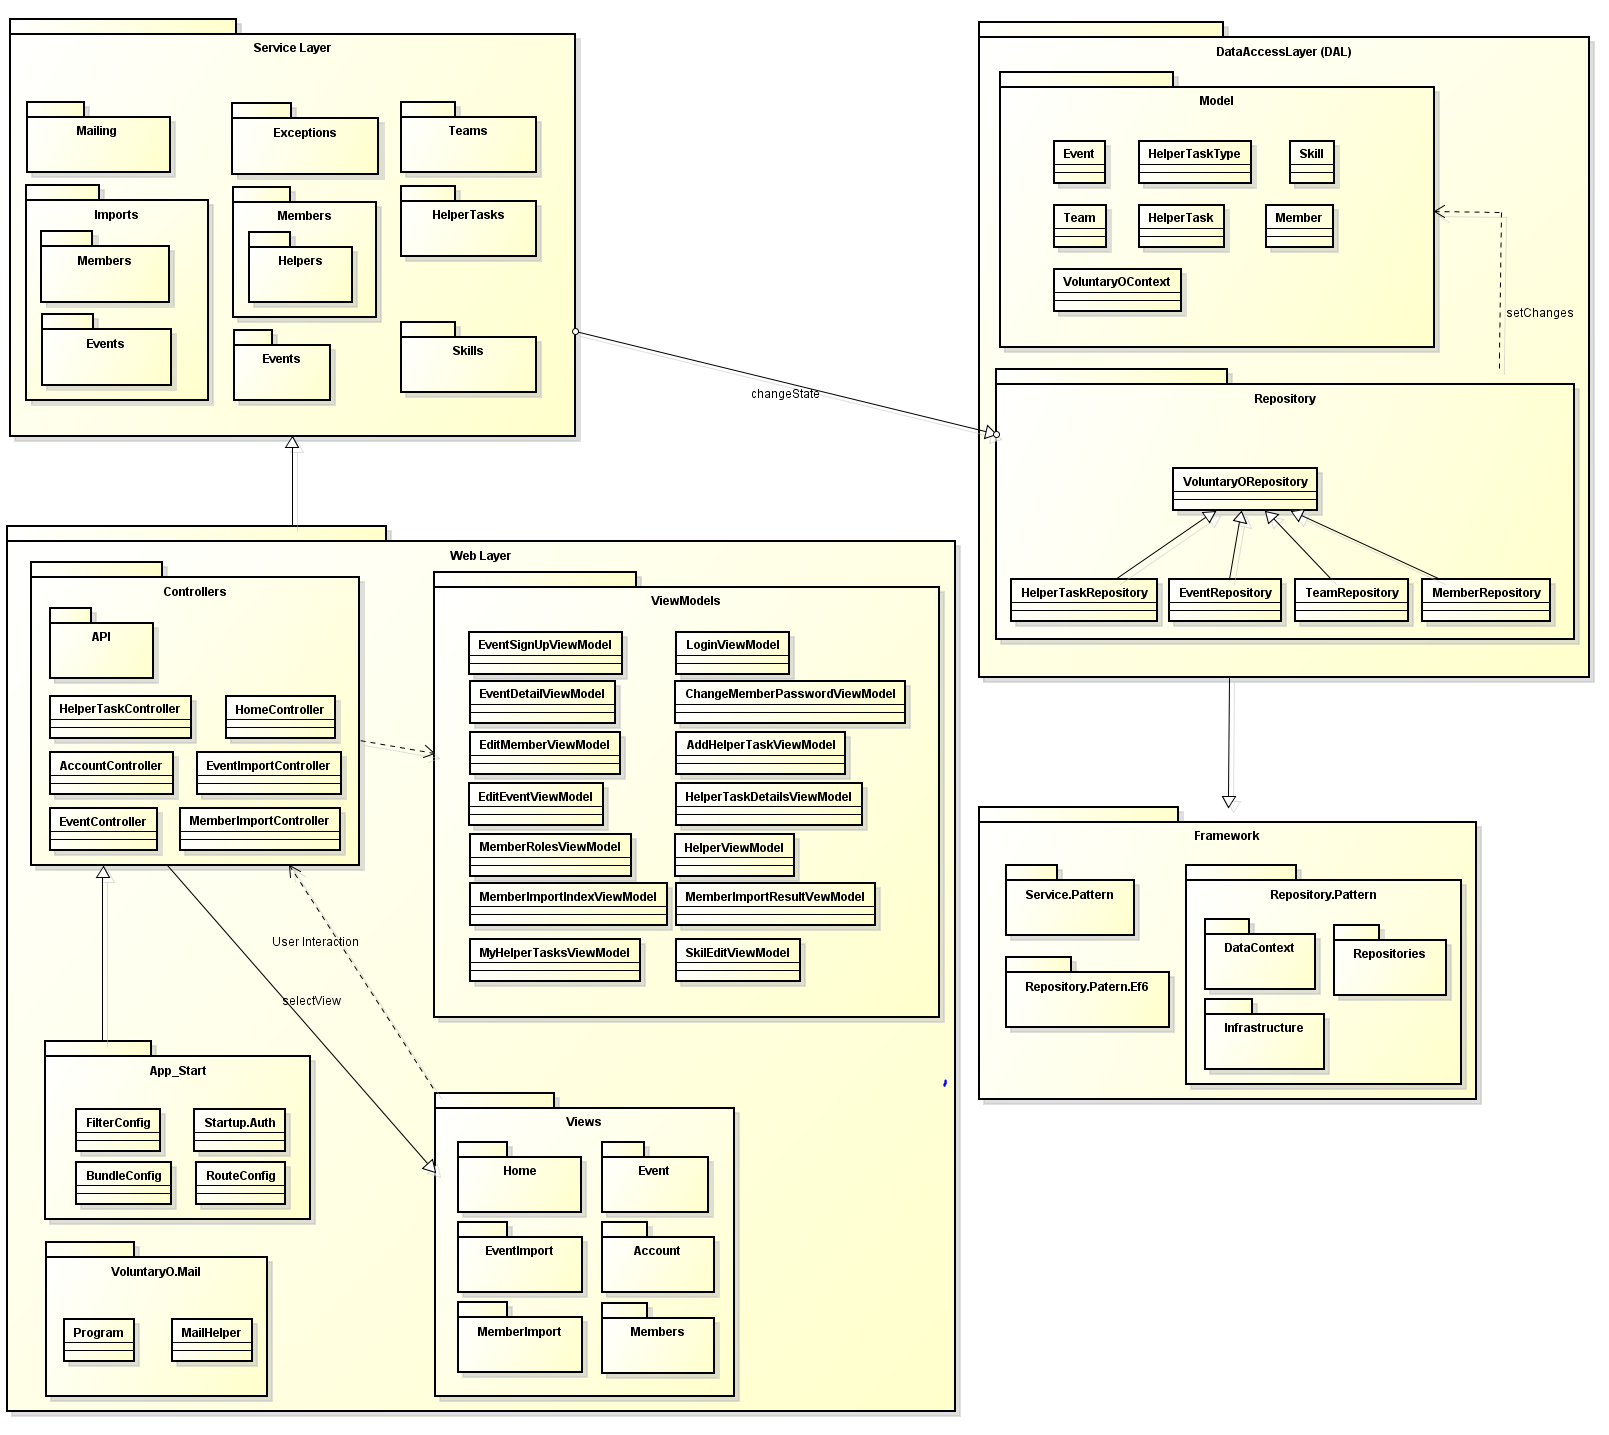
\includegraphics[width=\textwidth]{content/architekturdokumentation/images/LogischeArchitektur.png}

\section{VoluntaryO.Dal (Data Access Layer)}
    \begin{figure}[h]
  		\vspace{-5pt}
    	\centering
    	% VOLO-124
		% \includegraphics[width=\textwidth]{content/architekturdokumentation/images/domain.png}
  		\vspace{-25pt}
    	\caption{Domain in Subsystem VoluntaryO.Dal}
	\end{figure}
	Jede Model-Klasse implementiert die Schnittstelle \textit{IObjectState}, resp. leitet von der abstrakten Klasse \textit{Entity} ab.

	\subsection{Mapping}
	Das Mapping wird mit dem \textit{modelBuilder} des EF gesteuert. Bspw.
	\begin{lstlisting}[language=CSharp, caption=Mapping in VoluntaryoContext.cs, label=lst:mappingcontextcs, firstnumber=1]
// TeamEventMapping
modelBuilder.Entity<Team>()
    .HasMany(t => t.Events)
    .WithMany(e => e.Teams)
    .Map(mc =>
    {
        mc.MapLeftKey("TeamID");
        mc.MapRightKey("EventID");
        mc.ToTable("TeamEventMappings");
    });
    \end{lstlisting}

	\subsection{Vergleich für Objekte}
	Einzig für die Member-Klasse wurde die Vergleichsmethode (Equals) überschrieben. Folgende Attribute der Klasse sind relevant:
	\\\begin{itemize}
		\item \textit{UserName}
		\item \textit{Firstname}
		\item \textit{Lastname}
		\item \textit{Birthdate}
	\end{itemize}

	\subsection{Repository / Unit of Work Pattern}
	Generell wird das \href{https://genericunitofworkandrepositories.codeplex.com/}{\textit{Generic Unit of Work \& Repositories Framework}} befolgt um den Code Test- und Wartbar zu halten. Folgende Vorteile tun sich auf:
	\\\begin{itemize}	
		\item Austauschbarkeit ORM
		\item Testbarkeit
		\item Jeder Request hat eigene Unit of Work (siehe später Dependecy Injection)
		\item Reduktion der Datenbankabfragen, da nur noch über Unit of Work commited wird
		\item Generische Abfragen von Entitäten
	\end{itemize}
	Folgende Konventionen ergeben sich aus für das Projekt:
	\\\begin{itemize}
		\item Jede Entität implementiert \textit{IObjectState}
		\item Repository kann über \textit{partial Classes} erweitern werden
		\item Oder Repository Klassen implementieren \textit{IRepository} und erben von \textit{Repository}
	\end{itemize}

	\subsection{Unit Tests mit Effort}
	\href{https://effort.codeplex.com/}{\textit{Effort}} ist ein ADO.Net Provider und erstellt jeweils eine In-Memory Datenbank für das EF. Die temporäre Datenbank ermöglicht uns ein Testen des Codes, ohne Datenbankzugriffe zu mocken.
	\begin{lstlisting}[language=CSharp, caption=Verwendung Effort für Unit Tests in EffortTest.cs, label=lst:effortunittest, firstnumber=1]
		DbConnection Connection = DbConnectionFactory.CreateTransient();
		VoluntaryoContext VoluntaryoContext = new VoluntaryoContext(_Connection);
    \end{lstlisting}
    Den einzelnen Unit Tests steht so eine saubere und testbare Datenbank zur Verfügung.


\section{VoluntaryO.Service}

\section{VoluntaryO.Web}
